% !TEX root = main.tex
\section{Motivation}

Model Predictive Control (MPC) refers to the class of control strategies that design control actions by solving a finite horizon optimal control problem at each sampling instant. While each optimization gives a sequence of optimal control actions, only the first action is applied to the process. The same procedure is applied in the next time instance after receiving the updated value of the process state. MPC has shown to be successful in industrial applications since it is able to handle large number of states and control actions and automatically considers constraints in the optimization.

The optimization of each time instance uses a dynamic model of the process to predict the future states and find the optimal sequence of actions that satisfies all the constraints. The objective function of the optimization is usually linear or quadratic. The resulting optimization problem can be cast as a linear program (LP) or quadratic program (LP), respectively, if the dynamic model is linear. For hybrid models with linear dynamics in each mode, the optimization problem can be cast as a mixed integer linear or quadratic program (MILP/MIQP). 

 The main difference between MPC and conventional control is in the nature of the function that maps the measured outputs to control actions. The former computes such a function online but the latter pre-computes it off-line. The required online computations in MPC limits its applicability to slow processes: the sampling time should be large enough to allow enough time for solving the optimization and obtaining the optimal action for the next time instance. Moreover, the optimization solver needs to be certified for using MPC in safety critical applications.
 % while the  therefore that in the latter the control function is pre-computed off-line.
These issues can be tackled using \emph{Explicit MPC} under proper assumptions on the model, constraints and the objective function. Explicit MPC solves the optimization problem off-line over a bounded domain of the state variables by using multiparametric programming techniques. The output of Explicit MPC is the optimal control actions as an ?explicit? function of the states which is piecewise affine. This expands the class of systems being controlled by MPC strategies since the implementation requires only storing a lookup table of linear gains and performing an affine computation using the appropriate gains at each time instance. A survey on Explicit MPC can be found in \cite{Alessio2009}.\\
\begin{figure}[t]
	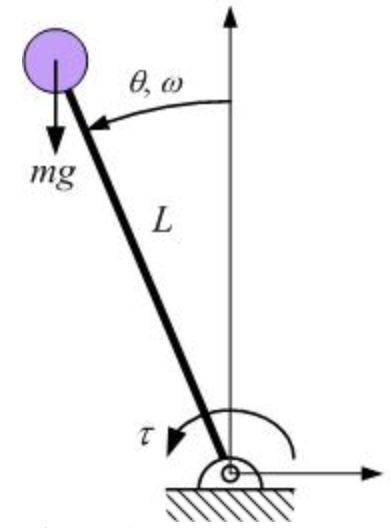
\includegraphics[width=3cm,height=5cm]{Figs/inv_pend.png}
	\label{fig:inverted_pendulum}
	\caption{Inverted pendulum}
\end{figure}
In this section, we use a classical control example to explain the motivation behind this work. Consider the problem of designing stablizing control for an inverted pendulum which takes (polytopic) constraints over state variables and control inputs into account. The linearized descrete-time description for the inverted pendulum depicted in Fig. \ref{fig:inverted_pendulum} is as follows:
	\begin{equation}
		\begin{bmatrix}
			 \theta_{k+1}\\
			\omega_{k+1}
		\end{bmatrix}=
		\begin{bmatrix}
			1 & T_s\\
			\frac{T_sg}{L}& (1-\frac{T_sb}{mL^2})		
		\end{bmatrix}
		\begin{bmatrix}
			\theta_k\\
			\omega_k
		\end{bmatrix}+
		\begin{bmatrix}
			0\\
			\frac{T_s}{mL^2}
		\end{bmatrix}u_k
		\label{eq:pendul_ss}
	\end{equation}
	where, $\theta$, $\omega$ and $u=\tau$ denote angular position, angular speed and input torque respectively; $g=9.81 m/s^2$ is the gravitational acceleration, $m$ the ball mass, $b$ the rotational fraction coefficient, $L$ the length of the bar and $T_s$ an appropriate sample time. Starting from an initial state, we would like the system's trajectory to converge into its equilibrium point while always $\theta\in[-\pi,\pi]$ and $\omega\in[-\pi/8,\pi/8]$. \\
	While there are many control schemes which can be used to stablize the system (e.g. LQR, state feedback), adding polytopic constraints, MPC schemes will be the best choice. 
	%In literature, many control schemes are proposed for stablizing the system around the equilibrium point. 
	%In order to design a controller which takes additional safety constraints are taken into account, model predictive control (MPC) schemes seem to be best candidate. 
	However, one major challenge for implementing model predictive controllers over embedded systems will be to solve MPC optimality problem within each time step. Since the system under consideration is LTI, one can use explicit MPC scheme proposed in [Bemporad:2002] which computes partitions over state space together with affine functions which are used to compute the optimal control input over their corresponding partition. For the inverted-pendulum example, the computed controller contains $12$, over each an affine function is provided for generating the control input.\\
	%To overcome this issue, in [Bemporad:2002], explicite MPC, a multi-parametric programming based approach is proposed for LTI systems. 
	In practice, EMPC will be implemented over relatively low-price embedded systems which have limited memory capacity and computational power. Computing the optimal control input can be efficiently done using for example binary tree search. However, the memory limit is more crucial as it increases proportional to the number of partitions.	Therefore, we would like to explore ways to reduce required memory for saving different coefficients corresponding to the controllers.
	On the other hand, most of the industrial embedded systems over which EMPC is implemented, only support fixed point arithmetic. Using fixed point arithmetic, will cause approximation error that is inversely proportional to the number of bits used for representing each variable. It is necessary to count for approximation error as it might lead into violation of the constraints. Therefore, one needs to formulate the problem as robust EMPC to count for disturbance input $|\delta|\leq \Delta$ which is summed up with the control input torque $u$ in each time step.\\ %Setting the number of bits for storing different variables, one can compute the upper bound for approximation error, $\bar\omega$.
	%However, we would like to achieve the minimum number of bits to reduce memory requirements.
	Overlay, we would like to design a robust explicit model predictive controller, taking errors resulted by fixed-point arithmetic into account and to come up with a minimal set of mixed precision assignments for all the coefficients that must be stored over the embedded system. Let us denote the total number of bits required for implementation of RMPC by $N_b$. Given the maximum memory budget denoted by $\bar N_b$, the overal goal will be to design a robust EMPC that (i) achieves performance objectives such as stability, safety and so on; (ii) it is implemented in a way that $N_b\leq \bar N_b$ while the error resulted by fixed-point arithmetic is smaller than the error bound $\Delta$. To that end, our approach is to start with an initial $\Delta$; design a robust explicit MPC controller with respect to $\Delta$ and to use state of the art fixed-point error analyzers to come up with the minimum total number of bits for storing the controller into the embedded system.\\
	
	Figure \ref{fig:overview} gives a high-level overview of our proposed setup. We start with definint the memory budget $\bar N_b$ and an initial error bound $\Delta_0$. Again, back to the inverted pendulum example, we choose $\bar N_b=6000$ and $\Delta_0=0$. To design robust explicit MPC for the error bound $\Delta$, MATLAB is run and the output controller is computed. Next, we ask Daisy to provide us with a mixed precision scheme respecting the error bound $\Delta=0$. However, $\Delta=0$ is not realizable as error resulted from fixed-point implementation is always greater than zero. Therefore, we go ahead and choose $\Delta=0.05$. Solving robust EMPC problem for the new disturbance bound gives the new controller. Next, we ask Daisy to provide us with fixed-point precision for all the parameters such that $\Delta=0.05$ is respected. The mixed precision scheme given by Daisy results in total number of bits $N_b=6084$ and since $N_b>\bar N_b$, we increase $\Delta$ again. Choosing $\Delta=0.1$, Daisy provides us with a mixed precision scheme with $N_b=5900$ for the correponding robust EMPC. As $N_b<\bar N_b$ the design goals are satisfied and the loop stops here. Surprisingly, the mixed precision implementation takes $11\%$ less memory comparing to the smallest uniform precision that respects $\Delta$. 
%	Using the output of Daisy, we are able to reduce memory requirements for the embedded systems up-to $20\%$ comparing to the case that uniform fixed-point precision is used.
	
	
	
	\tikzstyle{block} = [draw, rectangle, 
	minimum height=3em, minimum width=6em]
	\tikzstyle{sum} = [draw,  circle, node distance=1cm]
	\tikzstyle{input} = [coordinate]
	\tikzstyle{output} = [coordinate]
	\tikzstyle{pinstyle} = [pin edge={to-,thin,black}]
	\begin{figure*}[t]
		\begin{tikzpicture}[auto, node distance=2cm,>=latex',scale=1]
			\centering
			\node [block,scale=.8, pin={[pinstyle]above:$\Delta=\Delta_0$},
			node distance=5cm] (RMPC) {RMPC design (MATLAB)};
			\node[] (partitions) at (2.5,.5){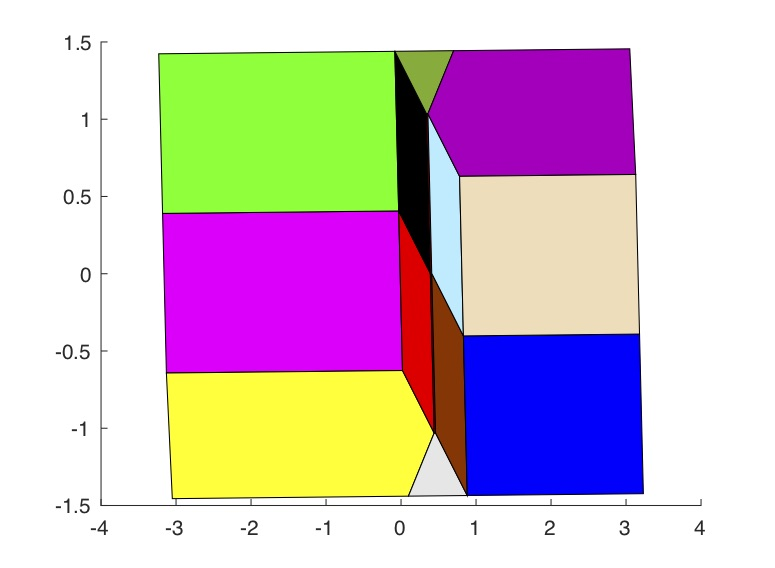
\includegraphics[width=.08\textwidth]{Figs/regs.jpg}};
			\node [block, scale=1,right of=RMPC,
			node distance=5cm,text width=3cm] (mixed) {Mixed precision computation (Daisy)};
			\node [draw, diamond, 
			minimum height=3em, minimum width=3em, right of=mixed,
			node distance=5cm] (decide) {$N_b\leq \bar N_b$};
			\node [block, right of=decide,
			node distance=3cm] (done) {Done};
			\node [block, below of= decide,
			node distance=3cm] (delta) {increase $\Delta$};
			\node [scale=.3] at (2.25,-.5)  {
				$
				K(x_k)=
				\begin{cases}
				F_1x_k+G_1 & \text{if $x_k\in \mathcal{R}_1$}\\
				F_2x_k+G_2 & \text{if $x_k\in \mathcal{R}_2$}\\
				\vdots\\
				F_Px_k+G_P & \text{if $x_k\in \mathcal{R}_P$}
				\end{cases} 
				$
			};
		\node at (7.5,-.35) {$N_b$};
			
			
			\draw [draw,->] (RMPC) -- node [pos=-.1] {}(mixed);
			\draw [->] (mixed) -- node [name=aaa] {}(decide);
			\draw [->] (decide) -- node [above,pos=.3] {Yes} (done);
			\draw [->] (decide) -- node[pos=0.99] {} 
			node [] {No} (delta);
			\draw [->] (delta) -| node [above] {} (RMPC);
	
	\end{tikzpicture}
	\caption{high-level description of the proposed memory-efficient robust MPC design}
	\label{fig:overview}
\end{figure*}

	